\documentclass{article}
\usepackage[T1]{fontenc}
\usepackage{lmodern}
\usepackage{graphicx}
\usepackage{amsmath,amssymb}
\usepackage[a4paper,margin=2cm]{geometry}
\usepackage[absolute,overlay]{textpos}
\setlength{\TPHorizModule}{1mm}
\setlength{\TPVertModule}{1mm}
\usepackage[indonesian]{babel}
\usepackage{hyperref}
\setlength{\emergencystretch}{2em}
% unit: Halaman 67

\begin{document}

% === Halaman 67 (llm) ===

\section*{Tantangan Masa Depan Kriptografi}

\vspace{143.75mm}

\begin{itemize}
    \item Lightweight cryptography
\end{itemize}

\vspace{60mm}

Sumber: \url{https://www.researchgate.net/figure/Lightweight-cryptographic-primitives-for-IoT_fig9_338830634}

% deskripsi: Diagram hierarki Lightweight Cryptography Primitives yang terbagi menjadi Lightweight Block Ciphers, Lightweight Stream Ciphers, Lightweight Hash Functions, dan ECC.
% bbox normalisasi: [0.0900, 0.3660, 0.8820, 0.8500]
\begin{textblock*}{166.32mm}(18.90mm,108.70mm)
\noindent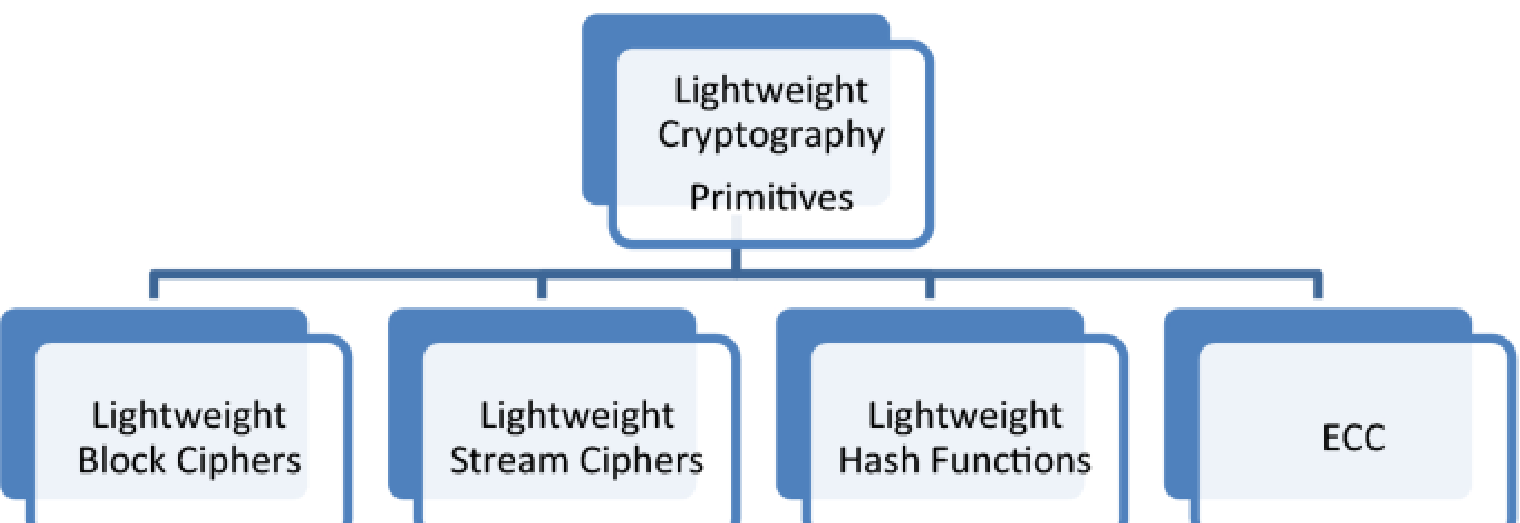
\includegraphics[width=166.32mm,height=143.75mm]{../../images/llm/page_067_img_01.png}%
\end{textblock*}

\end{document}
